\section{Problem Definition and Research Questions}
Recent advances on video generation models has raised the question of whether these models truly learn the physics of the world or simply replicate visual patterns \citep{liu2024sorareviewbackgroundtechnology}. At the same time, there is growing interest in leveraging video prediction for embodied control, with evidence that models trained on video and images can acquire useful knowledge for robot manipulation and navigation \citep{du2023learninguniversalpoliciestextguided, kim2024openvlaopensourcevisionlanguageactionmodel}. This motivates our study of whether video pretraining can lead to the acquisition of generalizable knowledge about environmental dynamics and how such knowledge can be leveraged for goal-directed behavior.

To study this in a controlled setting, we synthetically generate videos using a variation of the Game of Life \citep{gardner1970life} and build a simple game environment to test whether video pretraining helps agents navigate more effectively. We focus on grid-based environments of size $96 \times 96$, where agents must understand spatial structure and underlying transition dynamics. Our core research questions are:

\textit{\textbf{RQ1:} Does next frame prediction on videos enable a model to learn the underlying physics of an environment?}

We evaluate whether a model trained on video trajectories internalizes the transition dynamics of the environment, measured by its ability to generate accurate predictions on unseen initial configurations.

\textit{\textbf{RQ2:} Can knowledge acquired through video pretraining be leveraged to achieve goal-directed behavior more effectively?}

We test whether initializing a reinforcement learning agent from a pretrained video model leads to faster learning, fewer required interactions, or higher rewards compared to training from scratch.

\textit{\textbf{RQ3:} Does video pretraining support generalization across environments where the rules of physics change?}

We assess whether a model pretrained on diverse Game of Life variants can transfer its learned representations to environments with previously unseen rules.

\textit{\textbf{RQ4:} How can test-time training be integrated with reinforcement learning for continual adaptation to unseen environments?}

We explore whether an agent can adapt its internal representations at test-time to infer and adjust to new environment dynamics.

During the timeline of the project, as time allows, we will try to address the questions in order.
\section{Setup}
\begin{figure}[ht]
    \centering
    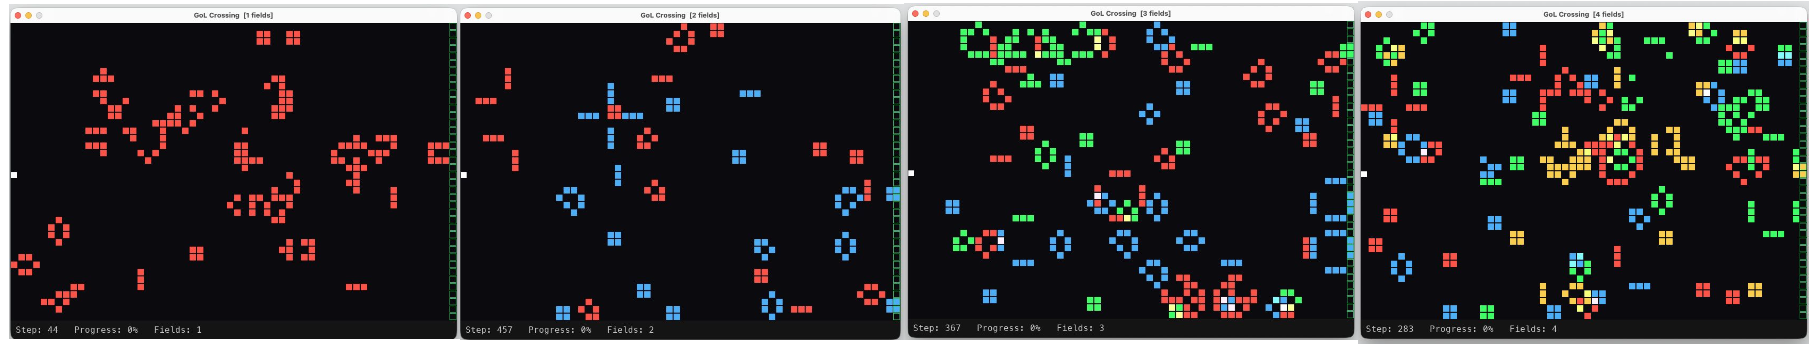
\includegraphics[width=0.8\linewidth]{Figures/Figure1.png}
    \caption{Example game environment setup. Each video frame serves as a training signal for synthetic video pretraining via next-frame prediction. The reinforcement learning agent is subsequently initialized from the pretrained model weights.}
    \label{fig:example}
\end{figure}
Our pipeline consists of two stages: (1)~self-supervised pretraining via next-frame prediction on synthetic videos, and (2)~reinforcement learning in the game environment using the pretrained model as initialization.

\subsection{Pretraining Dataset}

We construct a pretraining dataset of synthetic videos generated from a variation of Conway's Game of Life~\citep{gardner1970life}. To increase complexity beyond the standard binary cellular automaton, we run $K$ parallel Game of Life fields simultaneously and color-code each field in the rendered $96 \times 96$ RGB display. Videos are generated by simulating $T$ timesteps from random initial configurations, yielding a diverse corpus of trajectories with rich spatiotemporal dynamics. Using synthetic data provides a controlled setting with known ground-truth dynamics, enabling precise evaluation of whether the model has internalized the underlying transition rules.

\subsection{Frame Crossing Game}

We define a reinforcement learning task called the \textit{Frame Crossing Game}. The agent must navigate from one side of the grid to the opposite side in minimum time. The background consists of evolving Game of Life cells: contact with any active cell terminates the episode, while reaching the opposite boundary yields a positive reward. A per-step penalty encourages speed. Crucially, since the colored cells evolve according to Game of Life dynamics, the agent must anticipate future states to plan a safe trajectory, directly linking the pretraining objective to downstream task performance.